% Options for packages loaded elsewhere
\PassOptionsToPackage{unicode}{hyperref}
\PassOptionsToPackage{hyphens}{url}
%
\documentclass[
  ignorenonframetext,
]{beamer}
\usepackage{pgfpages}
\setbeamertemplate{caption}[numbered]
\setbeamertemplate{caption label separator}{: }
\setbeamercolor{caption name}{fg=normal text.fg}
\beamertemplatenavigationsymbolsempty
% Prevent slide breaks in the middle of a paragraph
\widowpenalties 1 10000
\raggedbottom
\setbeamertemplate{part page}{
  \centering
  \begin{beamercolorbox}[sep=16pt,center]{part title}
    \usebeamerfont{part title}\insertpart\par
  \end{beamercolorbox}
}
\setbeamertemplate{section page}{
  \centering
  \begin{beamercolorbox}[sep=12pt,center]{part title}
    \usebeamerfont{section title}\insertsection\par
  \end{beamercolorbox}
}
\setbeamertemplate{subsection page}{
  \centering
  \begin{beamercolorbox}[sep=8pt,center]{part title}
    \usebeamerfont{subsection title}\insertsubsection\par
  \end{beamercolorbox}
}
\AtBeginPart{
  \frame{\partpage}
}
\AtBeginSection{
  \ifbibliography
  \else
    \frame{\sectionpage}
  \fi
}
\AtBeginSubsection{
  \frame{\subsectionpage}
}
\usepackage{lmodern}
\usepackage{amssymb,amsmath}
\usepackage{ifxetex,ifluatex}
\ifnum 0\ifxetex 1\fi\ifluatex 1\fi=0 % if pdftex
  \usepackage[T1]{fontenc}
  \usepackage[utf8]{inputenc}
  \usepackage{textcomp} % provide euro and other symbols
\else % if luatex or xetex
  \usepackage{unicode-math}
  \defaultfontfeatures{Scale=MatchLowercase}
  \defaultfontfeatures[\rmfamily]{Ligatures=TeX,Scale=1}
\fi
\usetheme[]{Madrid}
% Use upquote if available, for straight quotes in verbatim environments
\IfFileExists{upquote.sty}{\usepackage{upquote}}{}
\IfFileExists{microtype.sty}{% use microtype if available
  \usepackage[]{microtype}
  \UseMicrotypeSet[protrusion]{basicmath} % disable protrusion for tt fonts
}{}
\makeatletter
\@ifundefined{KOMAClassName}{% if non-KOMA class
  \IfFileExists{parskip.sty}{%
    \usepackage{parskip}
  }{% else
    \setlength{\parindent}{0pt}
    \setlength{\parskip}{6pt plus 2pt minus 1pt}}
}{% if KOMA class
  \KOMAoptions{parskip=half}}
\makeatother
\usepackage{xcolor}
\IfFileExists{xurl.sty}{\usepackage{xurl}}{} % add URL line breaks if available
\IfFileExists{bookmark.sty}{\usepackage{bookmark}}{\usepackage{hyperref}}
\hypersetup{
  pdftitle={Methods for Selection Bias in the UK Biobank},
  pdfauthor={Valerie Bradley},
  hidelinks,
  pdfcreator={LaTeX via pandoc}}
\urlstyle{same} % disable monospaced font for URLs
\newif\ifbibliography
\usepackage{graphicx,grffile}
\makeatletter
\def\maxwidth{\ifdim\Gin@nat@width>\linewidth\linewidth\else\Gin@nat@width\fi}
\def\maxheight{\ifdim\Gin@nat@height>\textheight\textheight\else\Gin@nat@height\fi}
\makeatother
% Scale images if necessary, so that they will not overflow the page
% margins by default, and it is still possible to overwrite the defaults
% using explicit options in \includegraphics[width, height, ...]{}
\setkeys{Gin}{width=\maxwidth,height=\maxheight,keepaspectratio}
% Set default figure placement to htbp
\makeatletter
\def\fps@figure{htbp}
\makeatother
\setlength{\emergencystretch}{3em} % prevent overfull lines
\providecommand{\tightlist}{%
  \setlength{\itemsep}{0pt}\setlength{\parskip}{0pt}}
\setcounter{secnumdepth}{-\maxdimen} % remove section numbering
%\setbeamertemplate{navigation symbols}{}
%ß\setbeamertemplate{footline}[frame number]{}


%\title[Methods for Selection Bias in the UK Biobank]{Methods for Selection Bias in UKB}
\institute[University of Oxford]{University of Oxford, Department of Statistics}

\titlegraphic{
	\vspace{1cm}
	\includegraphics[width=3cm]{/Users/valeriebradley/Documents/Oxford/logos/ox_small_cmyk_pos_rect.png}
}

%\definecolor{oxfordblue}{rgb}{0.267, 0.412, 0.49}
\definecolor{oxfordblue}{rgb}{0, 0.129, 0.278}
\usecolortheme[named=oxfordblue]{structure}

\title{Methods for Selection Bias in the UK Biobank}
\author{Valerie Bradley}
\date{15 October 2019}

\begin{document}
\frame{\titlepage}

\begin{frame}{The UK Biobank}
\protect\hypertarget{the-uk-biobank}{}

\textbf{UK Biobank}

\begin{itemize}
\tightlist
\item
  Largest ever prospective health study
\item
  Includes genetic sequencing, blood tests, physical exams, health
  history questionnaire
\item
  500,000 participants aged 40-70 when recruited between 2006 and 2010
\end{itemize}

\textbf{UK Biobank imaging cohort}

\begin{itemize}
\tightlist
\item
  Subset of UKB participants recruited to undergo additional imaging
  exams
\end{itemize}

\textbf{Goal}: Study exposures and outcomes that affect aging
populations

\end{frame}

\begin{frame}{Selection bias in the UK Biobank}
\protect\hypertarget{selection-bias-in-the-uk-biobank}{}

\begin{center}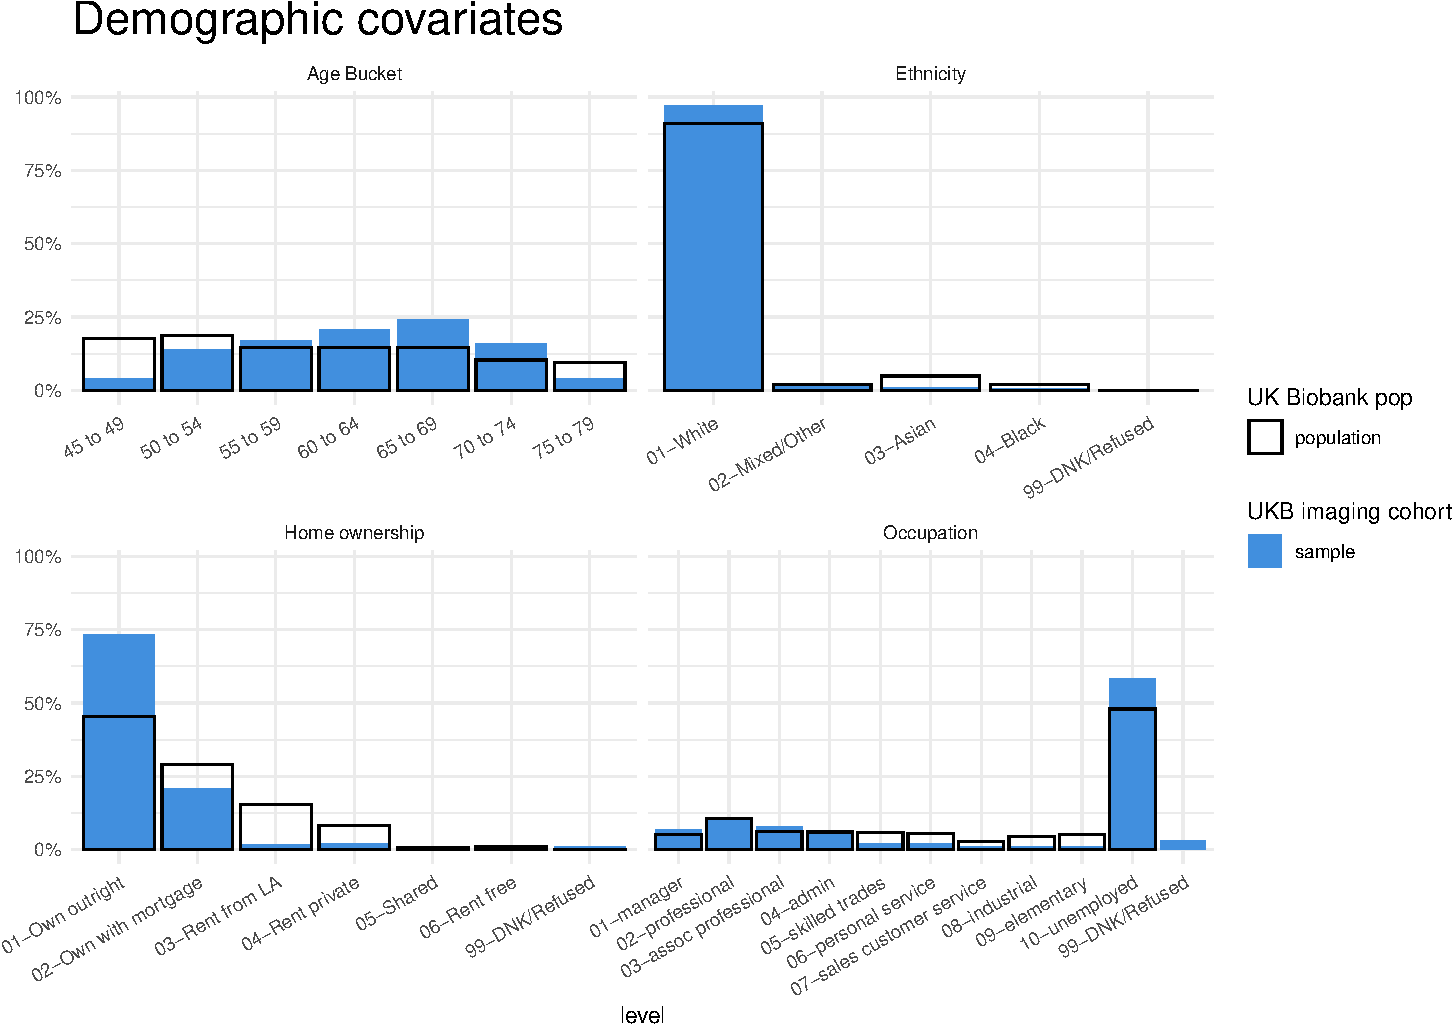
\includegraphics[width=0.95\linewidth]{fmrib-deck-20191002_files/figure-beamer/plot-selection-bias-demos-1} \end{center}

\end{frame}

\begin{frame}{Selection bias in the UK Biobank}
\protect\hypertarget{selection-bias-in-the-uk-biobank-1}{}

\begin{center}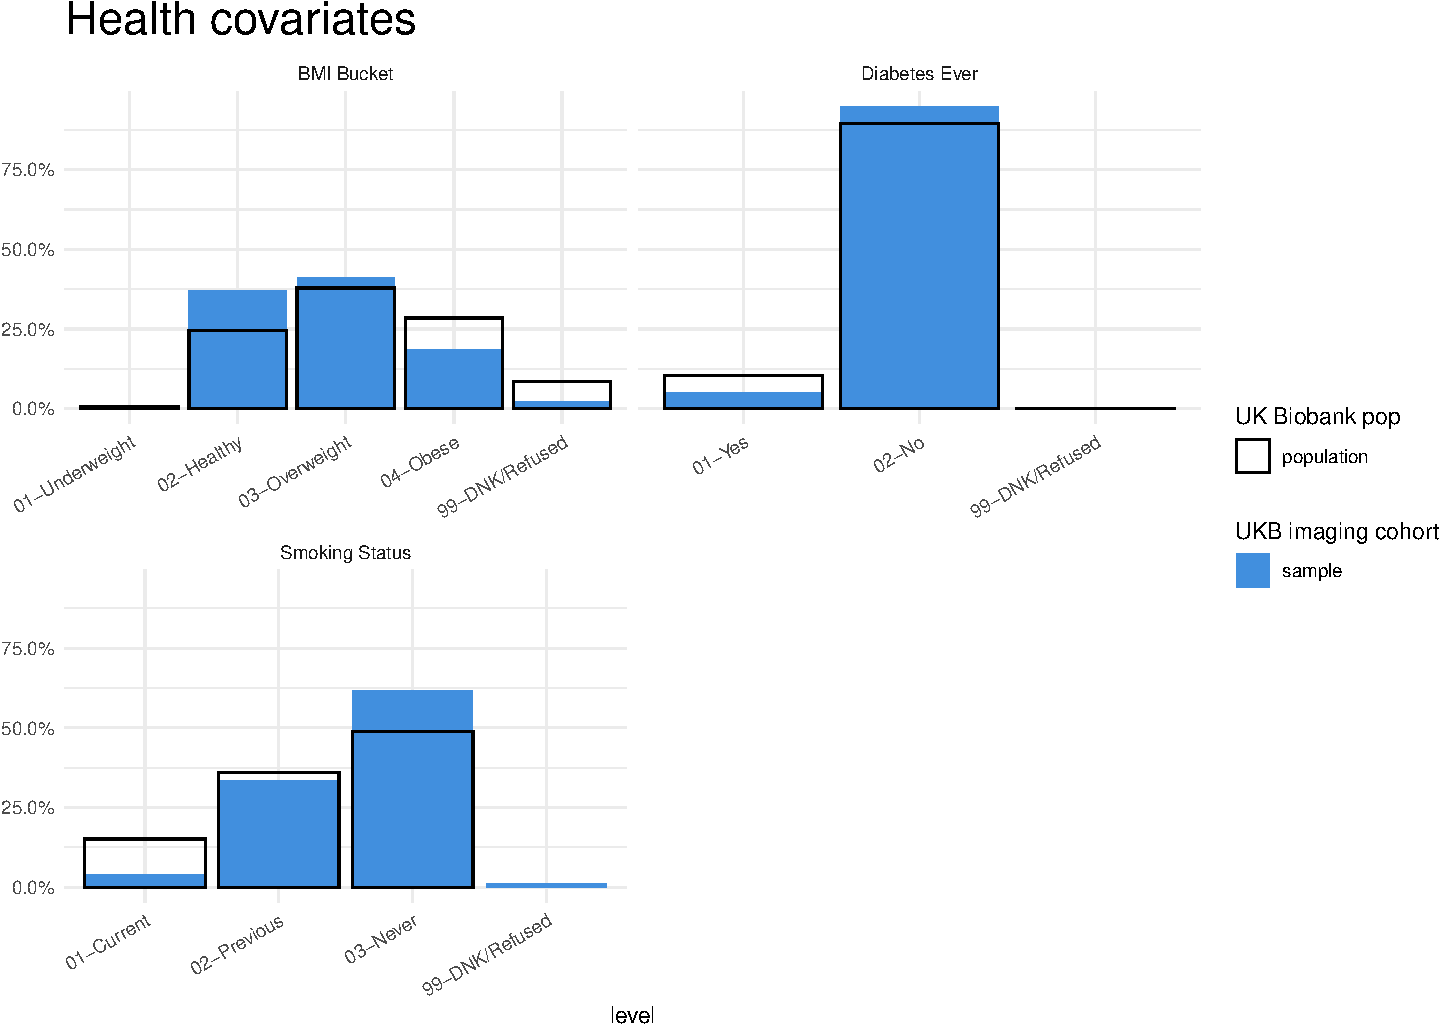
\includegraphics[width=0.95\linewidth]{fmrib-deck-20191002_files/figure-beamer/plot-selection-bias-health-1} \end{center}

\end{frame}

\begin{frame}{Why is this a problem?}
\protect\hypertarget{why-is-this-a-problem}{}

For example,

\begin{itemize}
\tightlist
\item
  Y is an individual's hippocampal volume
\item
  X represents a subject's socio-economic status (SES)
\item
  Z represents the subject's level of dementia
\item
  S is selection into the study
\end{itemize}

\center

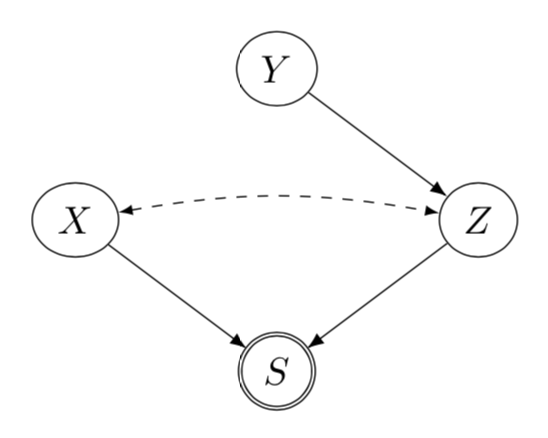
\includegraphics[width=0.4\linewidth]{~/github/mini-project-1/presentation/selection-bias-ex}
\center

By conditioning on selection, if we know that someone is of low SES,
they are less likely to show signs of dementia (than if we didn't know
their SES)

\end{frame}

\begin{frame}{Recovering from selection bias}
\protect\hypertarget{recovering-from-selection-bias}{}

If we can re-write our outcome of interest
\(\text{P}(\mathbf{y}|\mathbf{x})\) as

\(\text{P}(\mathbf{y}|\mathbf{x}) = \sum_\mathbf{z} \text{P}(\mathbf{y}|\mathbf{x}, \mathbf{z}, S=1)\text{P}(\mathbf{z}\setminus\mathbf{z^T}|\mathbf{z^T}, S = 1)\text{P}(\mathbf{z^T})\)

then it's possible to recover from selection bias.

\begin{itemize}
\tightlist
\item
  \(\mathbf{z}\) is a set of observed \emph{auxiliary variables}
\item
  \(\mathbf{z}^T\) is the subset of \(\mathbf{z}\) for which we have
  external, unbiased population data
\item
  Key is that conditioning on \(\mathbf{z}\) makes the outcome of
  interest, \(Y\), \emph{conditionally independent of selection}, \(S\)
\end{itemize}

\textbf{Problem}: can only condition on a limited number of discrete
variables before this breaks down

Methods for selection bias seek to solve this in different ways

\end{frame}

\begin{frame}{Methods: post-stratification}
\protect\hypertarget{methods-post-stratification}{}

\begin{block}{Intuition}

\end{block}

\end{frame}

\begin{frame}{Methods: summary}
\protect\hypertarget{methods-summary}{}

Classic weighting methods:

\begin{enumerate}
\tightlist
\item
  \emph{Post-stratification}: adjust to the joint distribution of
  \(\mathbf{z}\)
\item
  \emph{Raking}: iteratively adjust the marginal distributions of
  elements in \(\mathbf{z}\)
\item
  \emph{Calibration}: raking, but with continuous variables as well as
  discrete variables
\end{enumerate}

Less-common methods:

\begin{enumerate}
\setcounter{enumi}{3}
\tightlist
\item
  \emph{LASSO}: use a LASSO to select variables and interactions for
  raking
\item
  \emph{Logit}: estimate the probability of selection directly
\end{enumerate}

New method:

\begin{enumerate}
\setcounter{enumi}{5}
\tightlist
\item
  \emph{BART + raking}: use a BART to estimate the probability of
  selection, then rake such that key marginal distributions match those
  of the population
\end{enumerate}

\end{frame}

\begin{frame}{Simulation Results}
\protect\hypertarget{simulation-results}{}

\center

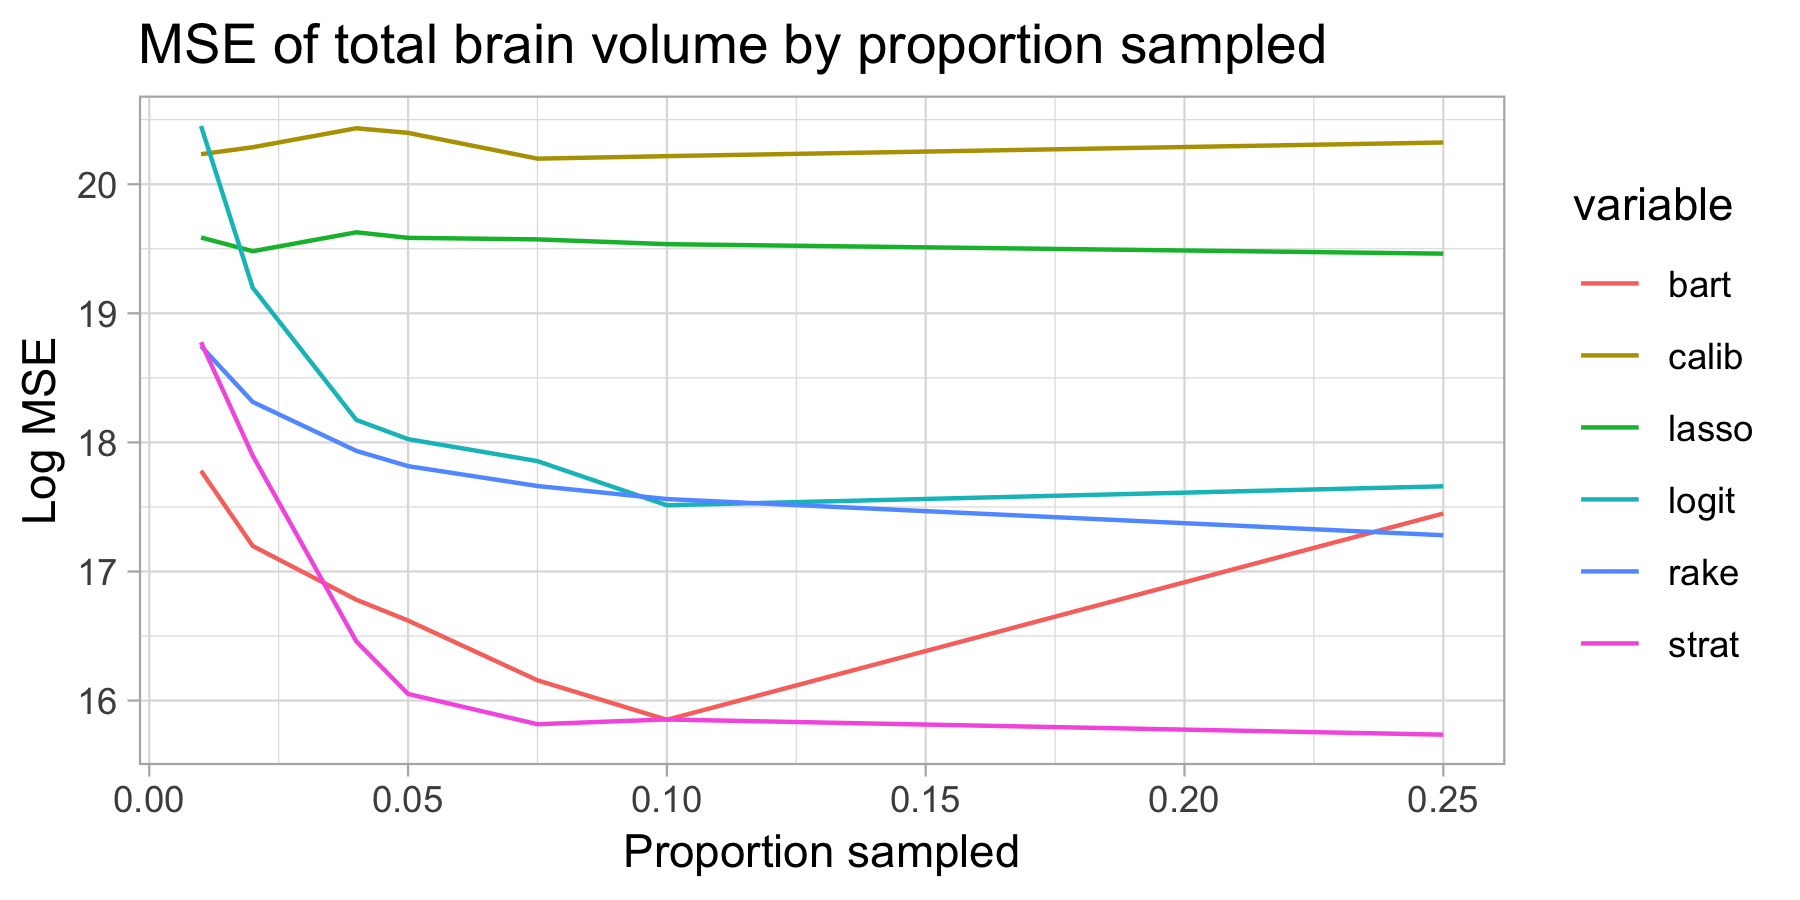
\includegraphics[width=1\linewidth]{~/github/mini-project-1/simulation/results/sim_1_5000_old_v3/plots/mse_by_sample_size}

\end{frame}

\begin{frame}{Application to UK Biobank}
\protect\hypertarget{application-to-uk-biobank}{}

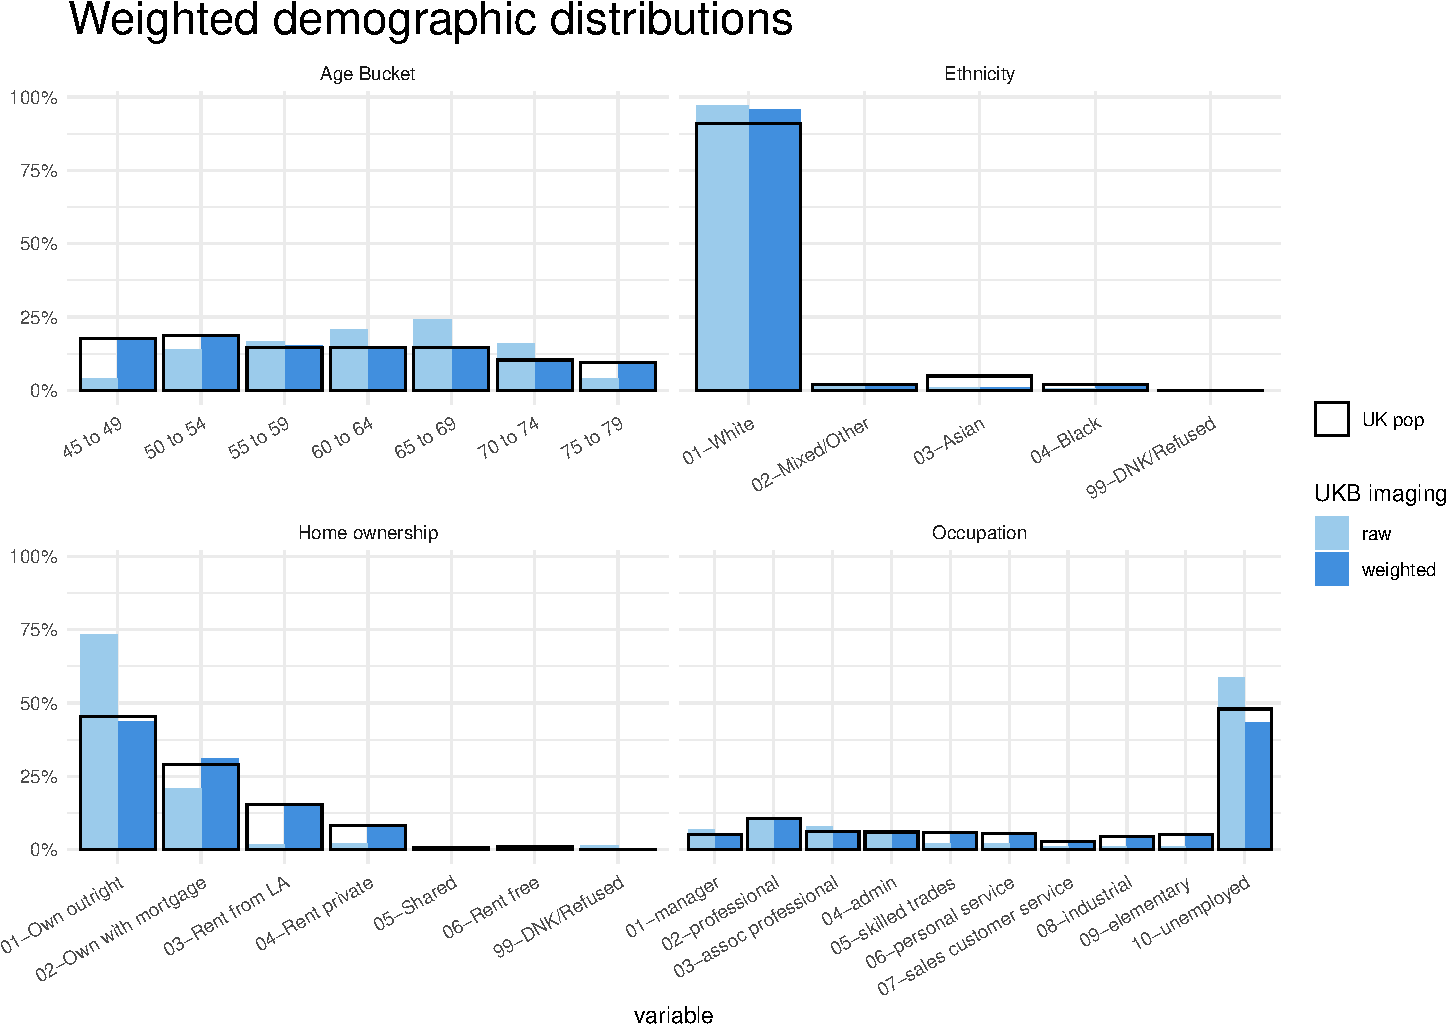
\includegraphics{fmrib-deck-20191002_files/figure-beamer/fig-ukb-results-1.pdf}

\end{frame}

\begin{frame}{Selection bias in the UK Biobank}
\protect\hypertarget{selection-bias-in-the-uk-biobank-2}{}

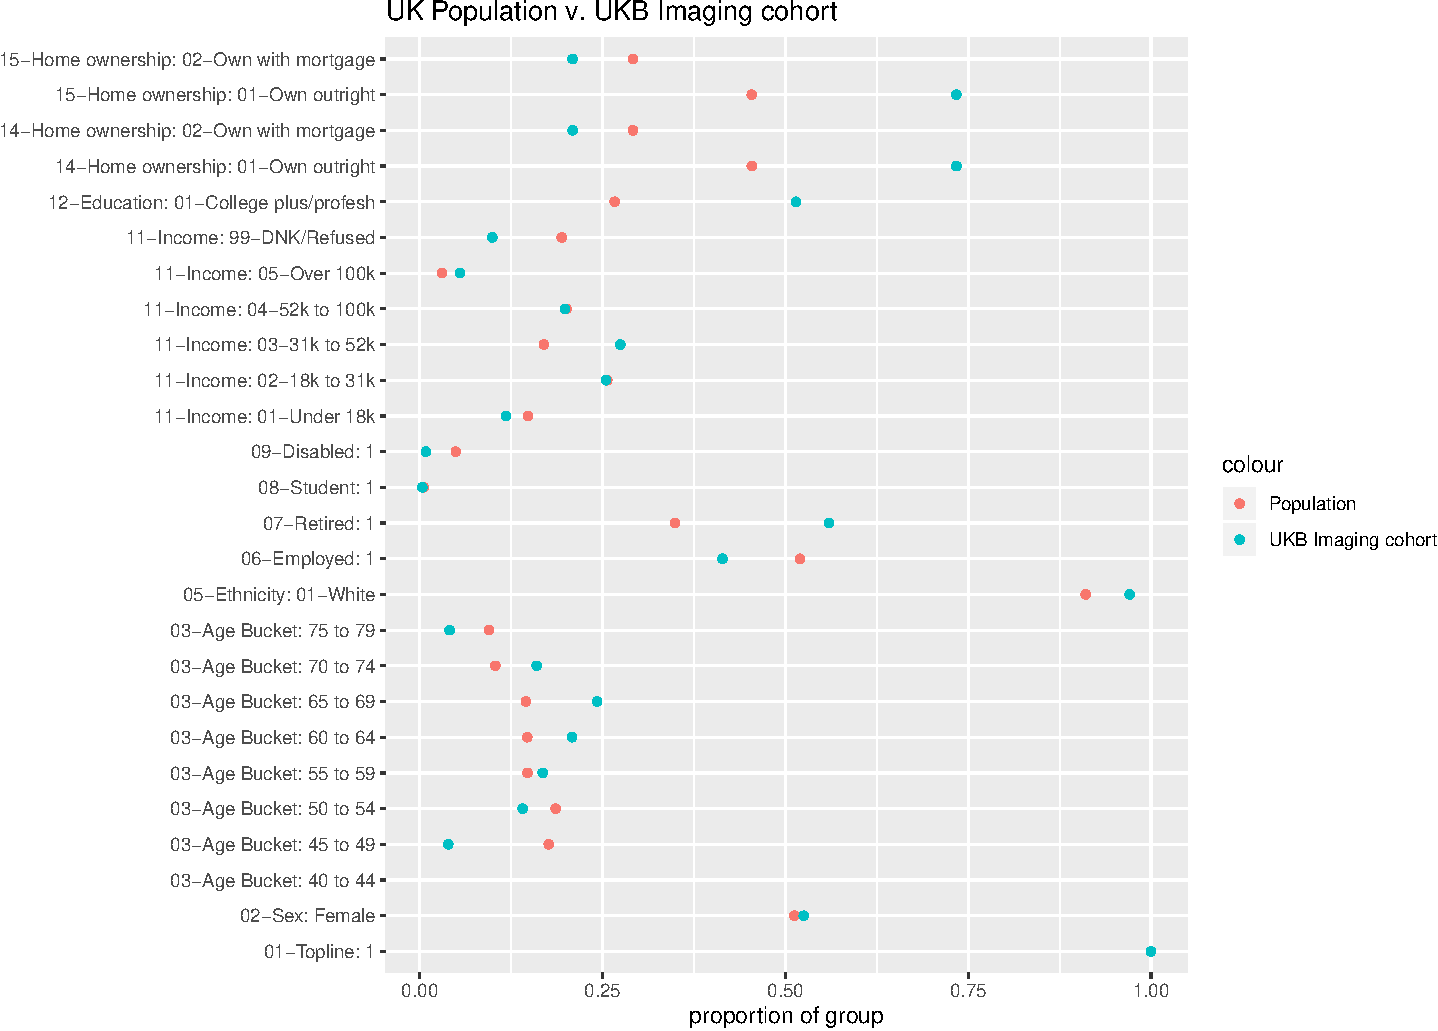
\includegraphics{fmrib-deck-20191002_files/figure-beamer/fig-1-1.pdf}

\end{frame}

\end{document}
